\section{Моделі та алгоритми для управління розподільчими логістичними системами}
\subsection{Основні принципи і допущення конфігурації логістичний мережі дистрибуції}
З метою вирішення завдання конфігурування логістичної мережі розглянемо основні принципи і допущення, які будуть використовуватися при формалізації структури дистрибутивної мережі ланцюжків постачань і вирішенні завдання структурного і параметричного синтезу. Будемо використовувати дві структурні розмірності мережі ланцюжків поставок: горизонтальну і вертикальну. Горизонтальна визначає число рівнів ланцюжків постачань, а вертикальна -- число ланок кожного рівня.

Логістична система дистрибуції будемо описувати у вигляді односпрямованого графа (рисунок~\ref{fig:log_structure}).

\begin{figure}[H]
	\centering
	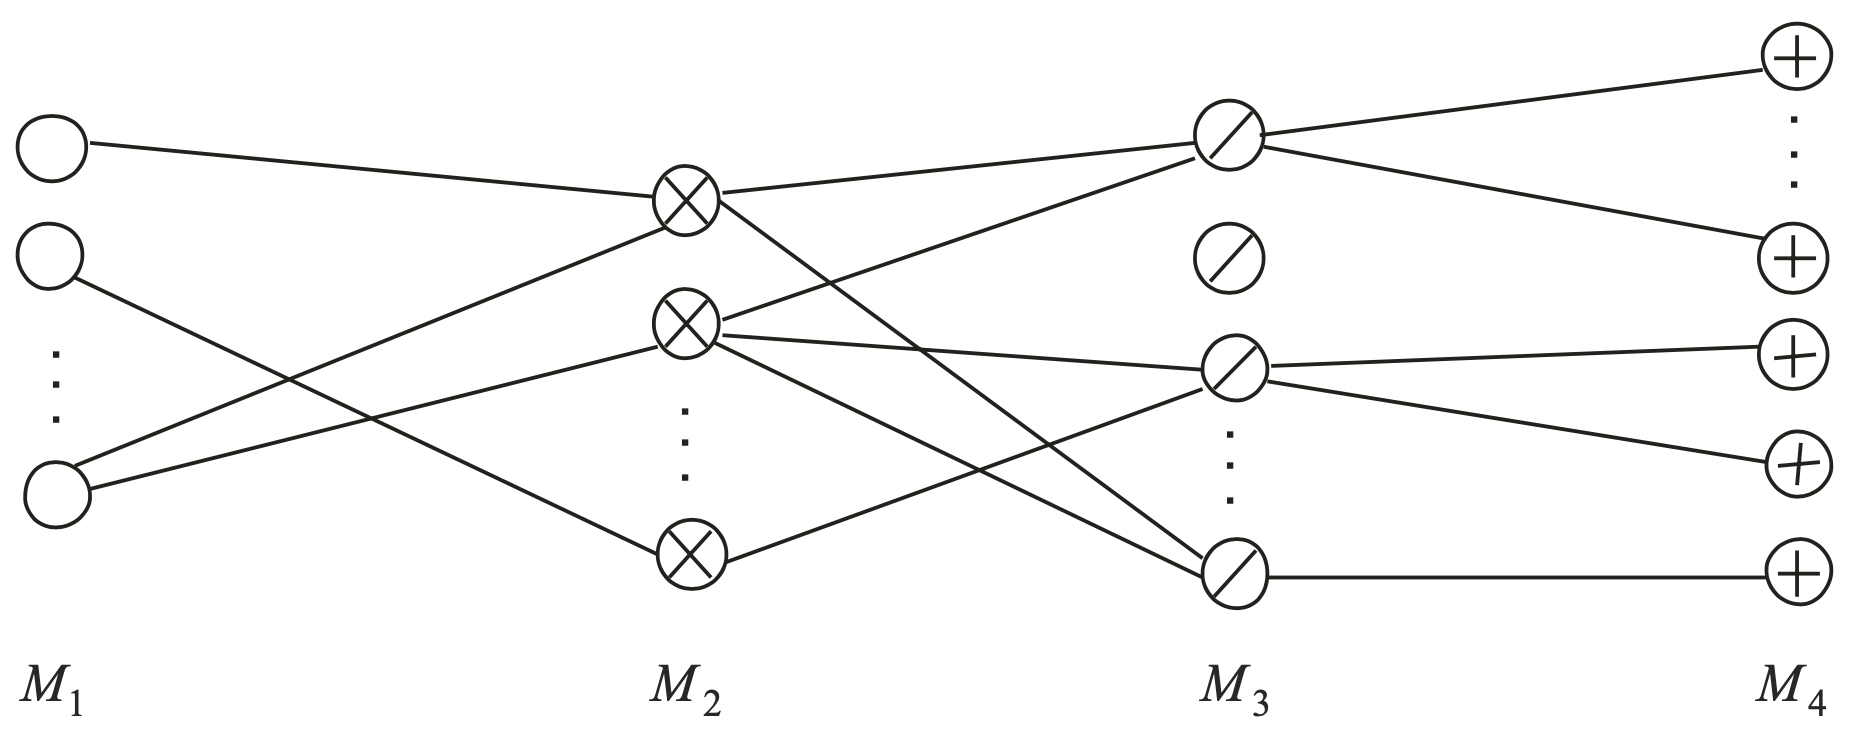
\includegraphics[width=0.7\textwidth]{log_structure}
	\caption{Структура логістичного каналу~\cite{Stankevich}}
	\label{fig:log_structure}
\end{figure}
\begin{description}
	\item[де] $M_1$ --- множина виробників продукції;
	\item $M_2$ --- множина центрів консолідації продукції (національні склади);
	\item $M_3$ --- множина центрів кастомізації продукції (регіональні склади);
	\item $M_4$ --- множина споживачів.
\end{description}

При стратегічному плануванні звичайно розглядається задача управління запасами з фіксованим циклом замовлень продукції.
Тому при заданій довжині циклу можна визначити об’єм продукції кожного виду.
На основі проведених досліджень~\cite{Stankevich} приймемо, що попит на кожний вид продукції має нормальний закон розподілу і довжина циклу однакова для всієї номенклатури і споживачів продукції. Тому можна записати вектор параметрів множини   нормальних законів розподілу попиту споживачів продукції:
\begin{equation}
	\alpha = \{ (\hat{\alpha}_{kp}, \check{\alpha}_{kp} ), k \in M_4, p \in P \},
\end{equation}
\begin{description}
	\item[де] $\hat{\alpha}_{kp}$ --- математичне очікування;
	\item $\check{\alpha}_{kp}$ --- середньоквадратичне відхилення для  $k$-го споживача та $p$-го виду продукції;
	\item $P$ --- множина видів продукції.
\end{description}

У роботі розглядається продукція масового використання з однаковим типом зберігання. Одиницею розмірності потоку перевезень є палета, у якій може бути розміщена різна кількість одиниць конкретних видів вантажу. Будемо вважати, що немає обмежень на сумісне перевезення різного виду вантажу. Тому зважаючи на незалежність випадкових величин попиту на продукцію різних видів, які мають нормальний закон розподілу, при виконанні центральної граничної теореми сумарний потік продукції може бути описаний випадковою величиною з нормальним законом розподілу і наступними параметрами~\cite{Stankevich}:
\begin{equation}
	\bar{\alpha}_k = \sum_{p\in P}\hat{\alpha}_{kp},\bar{\bar{\alpha}}_{kp} = \sqrt{\sum_{p \in P} (\check{\alpha}_{kp})^2}, k \in M_4,
\end{equation}
\begin{description}
	\item[де] $\bar{\alpha}_k$ --- математичне очікування сумарного потоку продукції для $k$-го споживача;
	\item $\bar{\bar{\alpha}}_{kp}$ --- середньоквадратичне відхилення величини сумарного потоку продукції для $k$-го споживача.
\end{description}

Попит на кожний $p$-й вид продукції множини $\bar{M}_{4j}$ є незалежною випадковою величиною.
Тому попит на $p$-й вид продукції $j$-го регіонального складу має нормальний закон розподілу з наступними характеристиками~\cite{Stankevich}:
\begin{equation} \label{eq:beta_hat}
	\hat{\beta}_{jp} = \sum_{k\in \bar{M}_{4j}} \hat{\alpha}_{kp}, p \in P, j \in \bar{M}_3,
\end{equation}
\begin{equation} \label{eq:beta_check}
	\check{\beta}_{jp} = \sqrt{\sum_{k\in \bar{M}_{4j}}(\check{\alpha}_{kp})^2} , p \in P, j \in \bar{M}_3,
\end{equation}
\begin{description}
	\item[де] $\hat{\beta}_{jp}$ --- математичне очікування нормального закону розподілу величини сумарного потоку продукції $p$-го виду у $j$-му регіональному складі;
	\item $\check{\beta}_{jp}$ --- середньоквадратичне відхилення нормального закону розподілу величини сумарного потоку продукції $p$-го виду у $j$-му регіональному складі.
\end{description}

Ці параметри відповідають фіксованій довжині циклу поставки продукції з регіональних складів на рівень первинних споживачів продукції. Якщо довжина циклу змінюється, то виконується корекція відповідних параметрів~\eqref{eq:beta_hat},~\eqref{eq:beta_check}.

При стратегічному плануванні ця задача розглядається з фіксованою довжиною циклу замовлень продукції~\cite{Stankevich}. Будемо вважати, що довжина циклу замовлень продукції зі складів її виробників на склади національного рівня дорівнює довжині циклу заказу продукції зі складів національного рівня на склади регіонального рівня. Крім цього, ці довжини дорівнюють $N$ довжинам циклу замовлень задачі розсіювання, де $N$ --- ціле число більше одиниці.

Вважаємо, що попит на продукцію у нашому випадку є стаціонарним процесом. Тому вірогідна величина потреби у $p$-му виді продукції на $j$-му регіональному складі при довжині циклу замовлень є вірогідною величиною з нормальним законом розподілу~\cite{Stankevich}. Тому його математичне очікування $\bar{\beta}_{jp}$ та середньоквадратичне відхилення $\bar{\bar{\beta}}_{jp}$ визначаються наступним чином~\cite{Stankevich}:
\begin{equation}
	\bar{\beta}_{jp} = N \cdot \hat{\beta}_{jp}, j \in \bar{M}_3, p \in P,
\end{equation}
\begin{equation}
	\bar{\bar{\beta}}_{jp} = \sqrt{(N \cdot \hat{\beta}_{jp})^2}, j \in \bar{M}_3, p \in P.
\end{equation}

У свою чергу на регіональних складах усі $P$ видів продукції є незалежними випадковими величинами. Крім цього, вони мають однаковий вид збереження продукції в палетах. Тому їх інтегрована величина також має нормальний закон розподілу з математичним очікуванням $\bar{\beta}_j^{\sum}$ та середньоквадратичним відхиленням $\bar{\bar{\beta}}_j^{\sum}$. Ці параметри нормального закону визначаються наступним чином~\cite{Stankevich}:
\begin{equation} \label{eq:b_2}
	\bar{\beta}_{j}^{\sum} = \sum_{p\in P} \bar{\beta}_{jp}, j \in \bar{M}_3,
\end{equation}
\begin{equation}
	\bar{\bar{\beta}}_{j}^{\sum} = \sqrt{\sum_{p\in P}(\bar{\bar{\beta}}_{jp})^2}, j \in \bar{M}_3.
\end{equation}

Інтегральний запас продуктів визначається величиною $\beta$, а потреба у ньому --- щільністю вірогідності з нормальним законом розподілу і параметрами $\bar{\beta}_j^{\sum}$, $\bar{\bar{\beta}}_j^{\sum}$. Математичне очікування $\bar{\beta}_j^{\sum}$ --- це середня потреба у запасі. На рис.~\ref{fig:log_bar} у якості прикладу розглядаються три варіанти страхового запасу, які відповідають одному, двом і трьом середньоквадратичним відхиленням.

\begin{figure}[H]
	\centering
	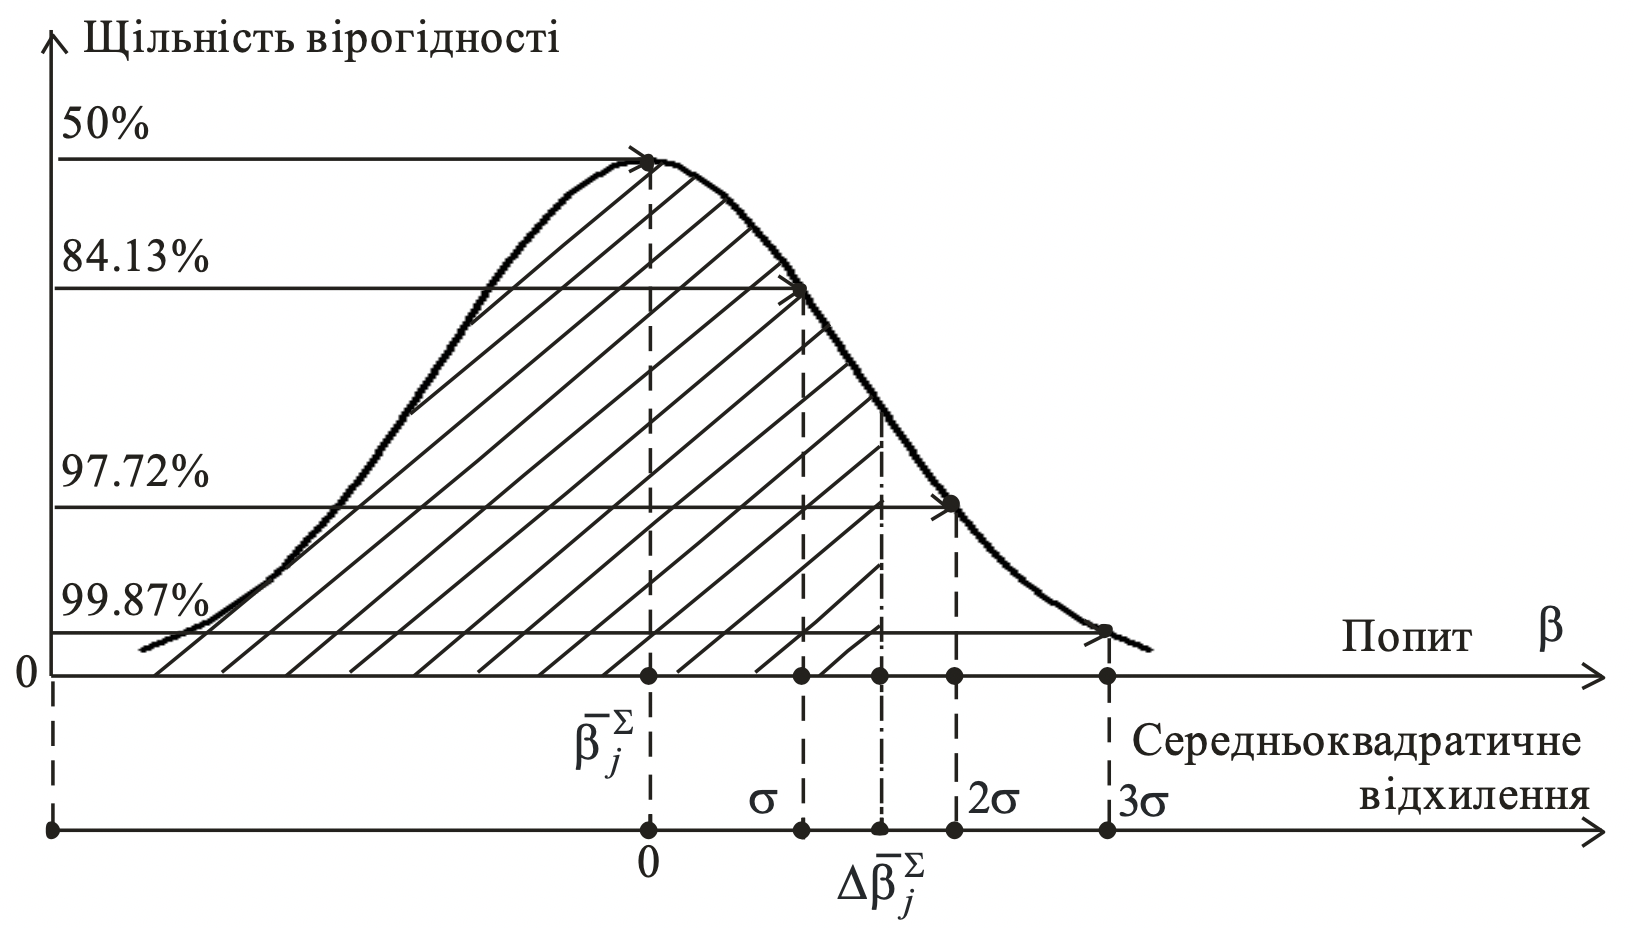
\includegraphics[width=0.7\textwidth]{log_bar}
	\caption{Щільність нормального закону розподілу попиту}
	\label{fig:log_bar}
\end{figure}

Праворуч від математичного очікування випадкової величини $\beta$ знаходиться область ризику дефіциту запасу, який виникає при задоволенні потреби у продукції, який перевищує середню величину (математичне очікування).
Ліворуч від математичного очікування випадкової величини $\beta$ знаходиться область ризику надлишків запасу продукції.
Площа, яка знаходиться під кривою функції щільності розподілу вірогідності в управлінні запасами є аналогом рівня сервісу.

Якщо страховий запас дорівнює нулю,а можливість зберігання продукції на $j$-му регіональному складі дорівнює величині $\bar{\beta}_j^{\sum}$, то базовий рівень сервісу обслуговування споживачів продукції дорівнює $50$\%. Якщо страховий запас дорівнює $\sigma$, то базовий рівень сервісу буде $84.13$\%. Для страхового запасу $2\sigma$ це $97.72$\%, а для $3\sigma$ --- $99.87$\%.

Таким чином, середньоквадратичне відхилення $\Delta\bar{\beta}_j^{\sum}$ є величиною страхового запасу для $j$-го регіонального складу, яка визначає рівень сервісу для споживачів.

Сформувати закон розподілу попиту для складів національного рівня по аналогії з регіональними складами неможливо, тому що один і той же регіональний склад обслуговується різними національними складами.
Тому запропоновано вважати, що сумарний об’єм страхового запасу для всіх складів національного рівня дорівнює сумарному страховому запасу регіонального рівня і для кожного складу національного рівня він є пропорційним величині $\bar{\beta}_j^{\Lambda}$, яка визначає сумарний об’єм ГП через $k$-й національний склад. Таким чином, об’єм страхового запасу для $k$-го національного складу визначається наступним чином:
\begin{equation} \label{eq:b_1}
	\Delta \bar{\beta}_k^{\Lambda} = \cfrac{\sum_{j \in \bar{M}_3} \Delta \bar{\beta}_j^{\sum} \cdot \bar{\beta}_j^{\Lambda} }{\sum_{j \in \bar{M}_2} \bar{\beta}^\Lambda_k }, k \in \bar{M}_2.
\end{equation}

Обсяг оренди складських приміщень дорівнює середньому обсягу ідеального попиту плюс страховий запас який рівний одному, двом або трьом среднеквадратическим відхиленням~\cite{Stankevich}.

\subsection{Розрахунок витрат на запаси}
Загальні витрати, пов'язані з запасами, представляють собою суму витрат на закупівлю, поповнення запасу і утримання запасів~\cite{Sterligova2008}:
\begin{equation} \label{eq:t}
T=C\cdot S+\cfrac{S}{C}\cdot A+(Z_s+\cfrac{Q}{2}\cdot I)
,
\end{equation}
\begin{description}
	\item[де] $T$ --- загальні витрати, пов'язані з запасом, г.~о.;
	\item $C$ --- закупівельні ціна одиниці товару, г.~о.;
	\item $Q$ --- розмір замовлення, одиниць;
	\item $S$ --- обсяг потреби в запасі, одиниць;
	\item $A$ --- витрати на виконання одного замовлення, г.~о.;
	\item $Z_s$ --- розмір страхового запасу, одиниць;
	\item $I$ --- витрати на утримання одиниці запасу, г.~о.
\end{description}

\subsection{Розрахунок оптимального розміру поповнення запасу}
В основі оптимізації рівня запасу лежить розрахунок розміру замовлення, який може забезпечити оптимальний рівень запасу при обслуговуванні на заданому рівні.
Критерієм оптимізації при цьому є, як правило, мінімум загальних витрат, пов'язаних з запасами.

Формула Вільсона --- найбільш відомий і широко вживаний метод розрахунку розміру замовлення~\cite{Sterligova2008}:
\begin{equation}
Q^*=\cfrac{dT}{dQ}=\sqrt{\cfrac{2\cdot A\cdot S}{I}}
,
\end{equation}
\begin{description}
	\item[де] $T$ --- загальні витрати~\eqref{eq:t}, пов'язані з запасом, г.~о.;
	\item $Q$ --- розмір замовлення, одиниць;
	\item $S$ --- обсяг потреби в запасі, одиниць;
	\item $A$ --- витрати на виконання одного замовлення, г.~о.;
	\item $I$ --- витрати на утримання одиниці запасу, г.~о.;
	\item $Q^*$ --- оптимальний розмір замовлення, одиниць.
\end{description}

\subsection{Модель з фіксованим інтервалом часу між замовленнями}
У моделі з фіксованим інтервалом часу між замовленнями  \textit{(fixed order interval model)} замовлення робляться в строго певні моменти часу, які знаходяться один від одного на рівні інтервали (рисунок~\ref{fig:model_fi:dynamic}).

\begin{figure}[H]
  \centering
\begin{tikzpicture}
  \begin{axis}[ 
    xlabel={Час},
    ylabel={Запас},
    xmin=0,xmax=10,ymin=0,ymax=1
  ] 
	\addplot
		coordinates {
			(0,0.8) [0]
			(3,0.2) [1]
			(3,0.8) [2]
			(7,0.25) [3]
			(7,0.9) [4]
			(9,0.1) [5]
			(9,0.8) [6]
			(10,0.5) [7]
		};
	\draw[<->] (axis cs:2.8,0.2) -- node[left]{\footnotesize $Q_i$} (axis cs:2.8,0.8);
   
    \draw [dashed] (axis cs:1.5,0) -- node[left]{\footnotesize Зам.} (axis cs:1.5,1);
    \draw [dashed] (axis cs:4.5,0) -- node[left]{\footnotesize Зам.} (axis cs:4.5,1);
    \draw [dashed] (axis cs:7.5,0) -- node[left]{\footnotesize Замовлення} (axis cs:7.5,1);

    \draw [densely dotted] (axis cs:0,0.4) -- node[below]{\footnotesize Пороговий запас} (axis cs:10,0.4);
    \draw [densely dotted] (axis cs:0,0.2) -- node[below]{\footnotesize Страховий запас} (axis cs:10,0.2);
  \end{axis}
\end{tikzpicture}
  \captionsetup{justification=centering}
  \caption{Динаміка запасу в моделі з фіксованим інтервалом часу між замовленнями}
  \label{fig:model_fi:dynamic}
\end{figure}

Розмір страхового запасу може бути розрахований різними методами.
Метод прямого рахунку~\cite{Sterligova2008}:
\begin{equation} \label{eq:model_fs:zs1}
Z_s=C_d-t_{od}
,
\end{equation}
\begin{description}
	\item[де] $C_d$ --- очікуване денне споживання, одиниць;
	\item $t_{od}$ --- час затримки постачання, дні.
\end{description}

Страховий запас визначається як різниця між максимальним споживанням під час виконання замовлення і очікуваним споживання під час виконання замовлення~\cite{Sterligova2008}:
\begin{equation} \label{eq:model_fs:zs2}
Z_s=MC-EC
,
\end{equation}
\begin{description}
	\item[де] $MC$ --- максимальне споживання за час виконання замовлення, одиниць;
	\item $EC$ --- очікуване споживання за час виконання замовлення, одиниць.
\end{description}

Формула для розрахунку інтервалу між замовленнями~\cite{Sterligova2008}:
\begin{equation} \label{eq:model_fi:time}
t_d=\cfrac{N\cdot Q^*}{S}
,
\end{equation}
\begin{description}
	\item[де] $t_d$ --- інтервал часу між замовленнями, дні;
	\item $N$ --- число робочих днів у плановому періоді, дні;
	\item $Q^*$ --- оптимальний розмір замовлення;
	\item $S$ --- обсяг потреби в запасі, одиниць.
\end{description}

Отриманий за допомогою формули~\eqref{eq:model_fi:time} інтервал часу між замовленнями не є обов'язковим.
Він може бути скоригований на основі експертних оцінок.

Максимальний бажаний запас визначається для відстеження доцільності завантаження площ складу з точки зору критерію мінімізації сукупних логістичних витрат.

Максимальний бажаний запас, як видно з рисунку~\ref{fig:model_fi:dynamic}, може бути розрахований таким чином~\cite{Sterligova2008}:
\begin{equation} \label{eq:model_fi:mws}
MWS=EC_t+Z_s
,
\end{equation}
\begin{description}
	\item[де] $MWS$ --- максимальний бажаний запас, одиниць;
	\item $EC_t$ --- очікуване споживання за інтервал часу між замовленнями;
	\item $Z_s$ --- обсяг страхового запасу, одиниць.
\end{description}

З урахуванням формули~\eqref{eq:model_fi:mws} розмір замовлення може бути розрахований за формулами~\cite{Sterligova2008}:
\begin{equation} \label{eq:order}
Q_i=EC_t+Z_s-Z_{Ti}-Z_t
,
\end{equation}
\begin{equation} \label{eq:order2}
Q_i=MWS-Z_{Ti}+EC-Z_{ti}
,
\end{equation}
\begin{description}
	\item[де] $Q_i$ --- розмір замовлення $i$, одиниць;
	\item $EC$ --- очікуване споживання за час виконання замовлення, одиниць;
	\item $Z_t$ --- обсяг запасу у дорозі, одиниць.
	\item $Z_{ti}$ --- обсяг запасу у дорозі, не отриманого до моменту видачі замовлення $i$, одиниць;
	\item $Z_{Ti}$ --- обсяг поточного запасу при видачі замовлення $i$, одиниць;
\end{description}

Страховий запас (формули~\ref{eq:model_fs:zs1},~\ref{eq:model_fs:zs2}) дозволяє задовольняти потребу в запасі на час передбачуваної затримки постачання.
При цьому під можливою затримкою постачання мається на увазі максимальна можлива затримка.

\subsection{Розрахунок рівня сервісу}
Розрахунок рівня логістичного обслуговування відбувається за наступною формулою~\cite{Sterligova2008}:
\begin{equation}
Y=\cfrac{m}{M} \cdot 100\%
,
\end{equation}
\begin{description}
	\item[де] $Y$ --- рівень логістичного обслуговування;
	\item $m$ --- кількісна оцінка фактично чиниться обсягу логістичних послуг;
	\item $M$ --- кількісна оцінка теоретично можливого обсягу логістичного сервісу.
\end{description}

\subsection{Метод ковзних середніх}
Метод ковзних середніх є одним з широко відомих методів згладжування часових рядів. Застосовуючи цей метод, можна елімінувати випадкові коливання і отримати значення, відповідні впливу головних чинників.

Згладжування за допомогою ковзних середніх засноване на тому, що в середніх величинах взаємно погашаються випадкові відхилення. Це відбувається внаслідок заміни первинних рівнів часового ряду середньою арифметичною величиною всередині обраного інтервалу часу. Отримане значення відноситься до середини обраного інтервалу часу (періоду).
Потім період зсувається на одне спостереження, і розрахунок середньої повторюється. При цьому періоди визначення середньої беруться весь час однаковими. Таким чином, в кожному даному випадку середня центрована, тобто віднесена до серединної точці інтервалу згладжування і являє собою рівень для цієї точки.

При згладжуванні часового ряду легкими середніми в розрахунках беруть участь всі рівні ряду. Чим ширше інтервал згладжування, тим більше плавним виходить тренд. Згладжений ряд коротше початкового на $(n-1)$ спостережень, де $n$ --- величина інтервалу згладжування.

При великих значеннях $n$ коливання згладженого ряду значно знижується. Одночасно помітно скорочується кількість спостережень, що створює труднощі.

Вибір інтервалу згладжування залежить від цілей дослідження. При цьому слід керуватися тим, в який період часу відбувається дія, а отже, і усунення впливу випадкових факторів.
Даний метод використовується при короткостроковому прогнозуванні. Його робоча формула:
\begin{equation} \label{eq:means}
	x_{t+1} = x_t \cdot f + x_{t - 1} (1 - f),
\end{equation}
\begin{description}
	\item[де] $x_{t+1}$ --- прогнозований показник;
	\item $x_{t-1}$ --- фактичне значення досліджуваного явища за попередній період;
	\item $x_{t}$ --- фактичне значення досліджуваного явища за поточний період;
	\item $f$ --- інтервалу згладжування.
\end{description}

\subsection{Координація дій агентів}
Моделі, методи та алгоритми взаємодії мультиагентних систем ґрунтуються на соціальних моделях~\cite{GerhardWeiss1996,Burkov}
Агенти у мультиагентних системах діють у навколишньому середовищі.
При значній чисельності агентів модель навколишнього середовища має передбачати інфраструктуру для колективної взаємодії агентів.
Ця інфраструктура має містити протоколи спілкування та взаємодії агентів між собою.

Протоколи спілкування дають змогу агентам обмінюватися та розуміти повідомлення.
Протоколи взаємодії забезпечують спілкуватися у вигляді структурованого обміну повідомленнями. Наприклад, протоколи спілкування можуть специфікувати такі типи повідомлень, які один агент може передати іншому~\cite{Fipa}:
\begin{itemize}
	\item пропозиція напрямку дій;
	\item згода або незгода з напрямком дій;
	\item відмова напрямку дій;
	\item корегування напрямку дій;
	\item вироблення іншої позиції щодо напрямку дій.
\end{itemize}

Систематика різних способів координації поведінки та активності агентів зображена на рисунку~\ref{fig:agent_coordination}.

\begin{figure}[H]
	\centering
	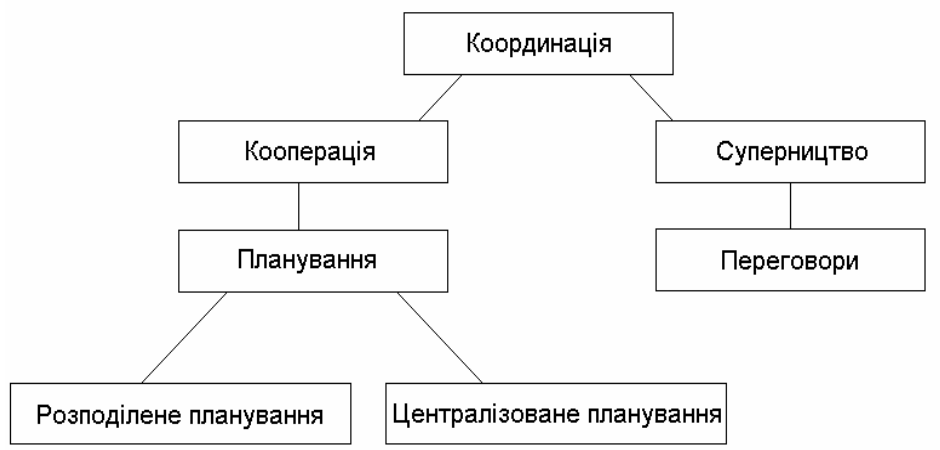
\includegraphics[width=0.7\textwidth]{agent_coordination}
	\caption{Способи координації поведінки агентів~\cite{GerhardWeiss1996}}
	\label{fig:agent_coordination}
\end{figure}

Спілкування агентів здійснюється на основі комунікаційного протоколу. Він має бути лаконічним, універсальним та спільним для всіх агентів.

\subsection{Визначення та типи агентів}
Схема агентів системи представлена на рисунку~\ref{fig:agent_scheme}.

\begin{figure}[H]
	\centering
	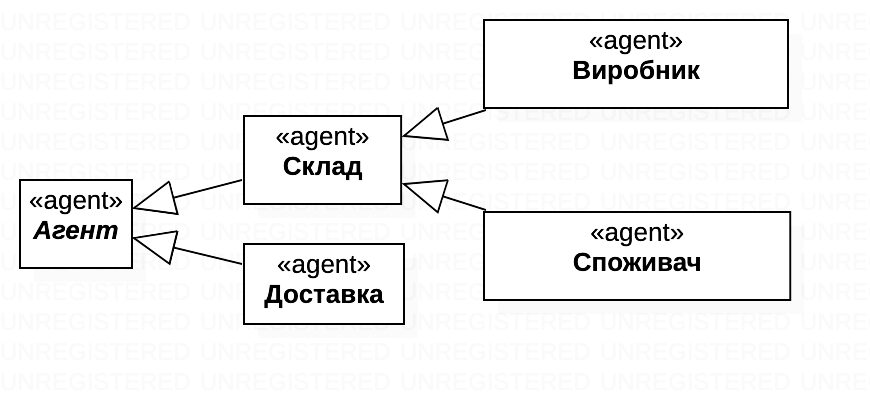
\includegraphics[width=0.6\textwidth]{agent_scheme}
	\caption{Схема агентів та моделей системи}
	\label{fig:agent_scheme}
\end{figure}
\begin{description}
	\item[де] склад --- базовий агент який реалізує можливість постачання та зберігання товарів, реагує на зміну кількості товарів;
	\item виробник --- симулює поведінку виробників продукції (рисунок~\ref{fig:log_structure});
	\item споживач --- симулює поведінку споживачів продукції (рисунок~\ref{fig:log_structure}).
\end{description}

Якщо агент просто своєчасно реагує на зміни зовнішнього середовища і реактивно перетворює свої сенсори на дії, цей агент реактивний.
Агенти які мають внутрішній стан та передбачають наслідки своїх дій називаються дорадчим агентом.

На рисунку~\ref{fig:agent_reactive} зображена схема реактивного агента. 
На рисунку~\ref{fig:agent_deliv} зображена схема дорадчого агента.

\begin{figure}[H]
	\centering
	\begin{subfigure}[b]{0.49\textwidth}
		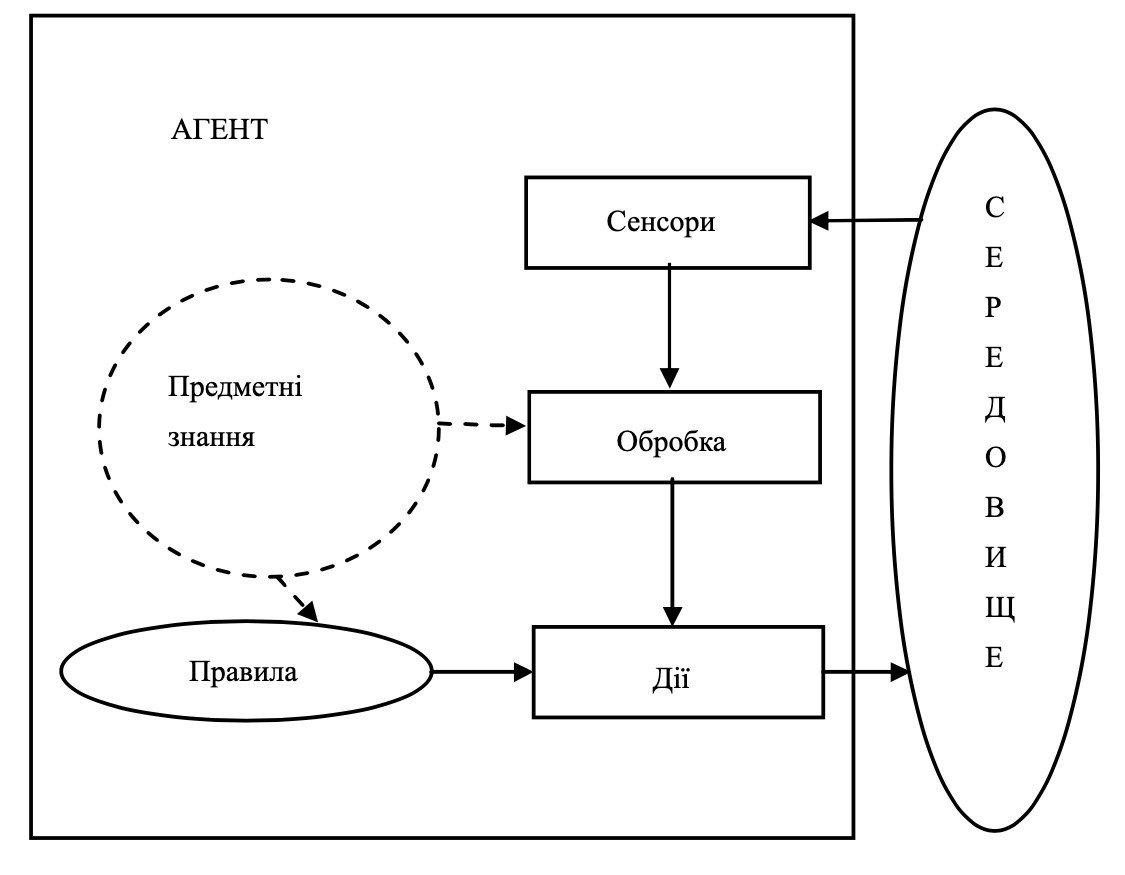
\includegraphics[width=\linewidth]{agent_reactive}
		\caption{Схема реактивного агенту}
		\label{fig:agent_reactive}
	\end{subfigure}
	~
	\begin{subfigure}[b]{0.49\textwidth}
		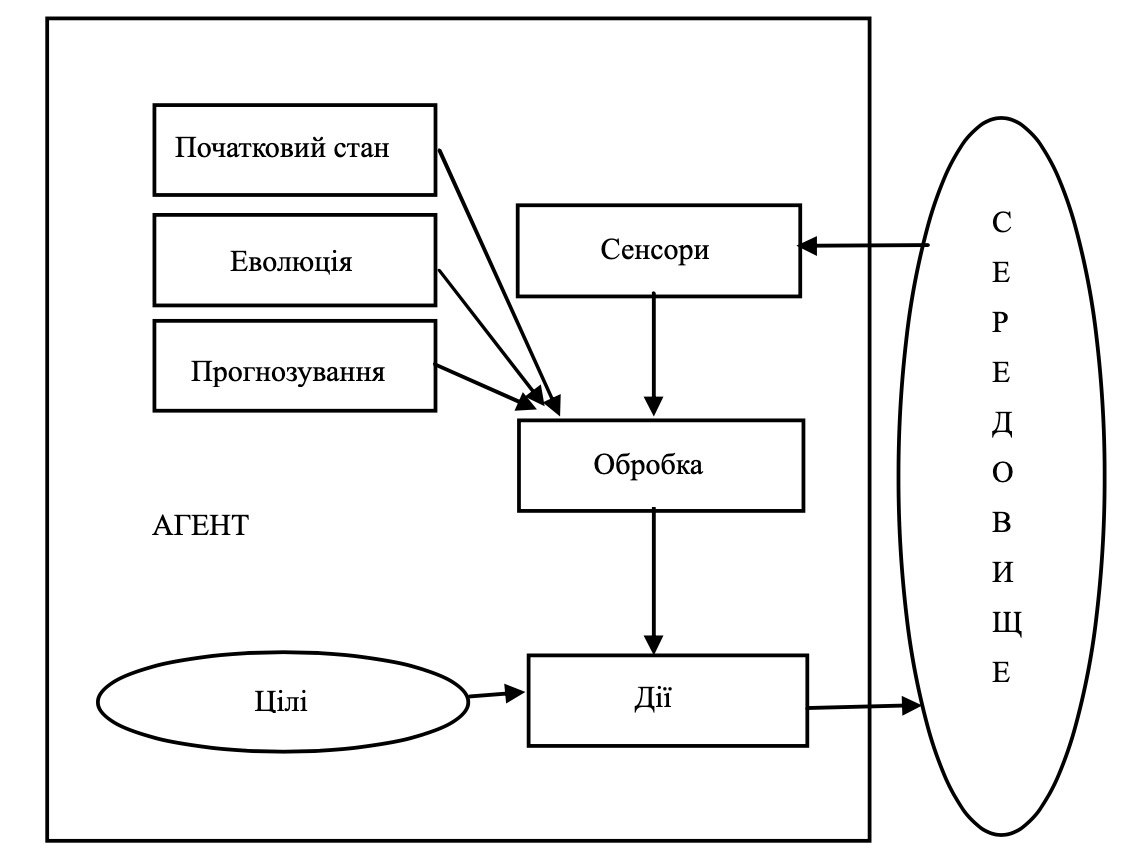
\includegraphics[width=\linewidth]{agent_deliv}
		\caption{Схема дорадчого агенту}
		\label{fig:agent_deliv}
	\end{subfigure}
    \caption{Порівняльна схема агентів}
\end{figure}

Оскільки доречним буде мати можливість прогнозування рівню запасів, то було прийнято рішення використовувати дорадчі агенти.

Цілями кінцевих агентів системи є:
\begin{enumerate}
	\item Зменшити вартість зберігання запасу, замовляючи ретельно розраховану кількість товарів;
	\item Недопустити вичерпання запасу;
	\item Доставка товарів без затримок.
\end{enumerate}

Формальна схема агенту складу представлена на рисунку~\ref{fig:agent_mine}.

\begin{figure}[H]
	\centering
	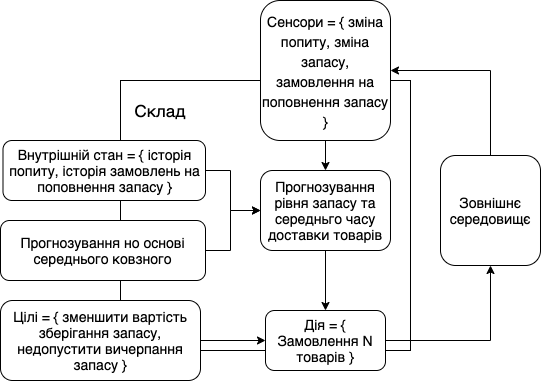
\includegraphics[width=0.7\textwidth]{agent_mine}
	\caption{Схема агенту складу}
	\label{fig:agent_mine}
\end{figure}

Склад має заданий об'єм який розраховується за формулами~\eqref{eq:b_2},~\eqref{eq:b_1}.

Агент складу реагує на таки зміни в навколишньому середовищі як:
\begin{itemize}
	\item зміна попиту;
	\item зміна запасу;
	\item замовлення на поповнення запасу.
\end{itemize} 

На основі історії попиту склад прогнозує рівень запасу та середнього часу доставки товарів з огляду на цикл замовлень. Прогнозування рівня запасу робиться за допомогою рівня середніх ковзних.

Агент замовляє товар, так щоб його вистачило до наступного циклу поставки товарів. 
